\chapter{Das Cherenkov Telescope Array}
\label{ch:CTA}
Mit dem Bau des Cherenkov Telescope Arrays (CTA) werden verschiedene Ziele verfolgt \cite{NextGen}:
\begin{itemize}

\item Abdeckung des Energiebereichs von 30GeV bis 100TeV
\item Verbesserung der Sensitivität um eine Größenordnung im Vergleich zur aktuellen Generation (H.E.S.S., VERITAS und MAGIC)
\item Verbesserung der Winkelauflösung auf $0,1^{\circ}$ bei 0,1TeV und $0,05^{\circ}$ bei 1TeV
\item Verbesserung der Energieauflösung auf 25\% bei 50GeV und 10\% bei 1TeV
\item Entdeckung einer großen Anzahl von Quellen bekannter Klassen
\item Entdeckung neuer Quellen (zum Beispiel Quellen GRBs)
\item Abdeckung des gesamten (nördlichen und südlichen) Himmels
\end{itemize}

\section{Design-Konzept}
Um die oben genannten Ziele zu erreichen, hat man sich für ein Arraykonzept entschieden, dass aus drei unterschiedlich großen Teleskoptypen besteht und an zwei Standorten errichtet wird.

\subsection{Teleskoptypen}
Für das CTA werden drei Teleskope unterschiedlicher Größe entwickelt, die in Abbildung \ref{img:TelescopeTypes} zu sehen sind.
\begin{description}
\item[Small Sized Telescope (SST)]\hfill \\
Das kleinste Teleskop ist sensitiv im Bereich von 1TeV bis 300TeV und wird eingesetzt um Schauer mit Energien über $\unit{TeV}$ zu detektieren. Momentan werden drei verschiedene Varianten entwickelt, die zu einem harmonisiert werden sollen. Das SST 1M ist eine kleinere Variante des MST und SST-2M  ASTRI und das SST-2M GCT basieren auf dem Prinzip eines Schwarzschild-Couder Designs. Das SST soll einen Reflektordurchmesser von ca. 4m haben.
\item[Medium Sized Telescope (MST)]\hfill \\ 
Das MST basiert auf einem modifiziertem Davies-Cotton-Design und hat einen Durchmesser von 12m. Mit einem Sensitivitätsbereich von 150GeV bis 5TeV deckt es den Kernbereich des CTAs ab. Ein Prototyp des MST wird in Berlin-Adlershof getestet.
\item[Large Sized Telescope (LST)]\hfill \\
Die größten Teleskope des CTA werden einen Reflektordurchmesser von 23m haben um auch Strahlung niedriger Energie zu detektieren. Um das Teleskop möglichst schnell zu bewegen, wurde durch den Einsatz von kohlefaserverstärktem Kunststoff Gewicht gespart. Das hat den Vorteil, dass die Teleskope zwar leichter werden, aber es hat auch den Nachteil, dass die Bauteile durch Bewegung des Teleskops stärker verbiegen, was das Pointing erschwert. Aufgrund der Größe dieser Teleskope reicht es nicht mehr den Reflektor dieser Teleskope sphärisch zu bauen, sondern parabolisch.% Hierbei steigt der Aufwand, da jeder einzelne Spiegel eine individuelle Brennweite hat.
\end{description}
\begin{figure}[htbp]
\centering
\includegraphics[width=\textwidth]{Images/TelescopeTypes.jpg}
\caption{Die drei verschieden großen Teleskope des CTA: links die drei Varianten des SMT, in der Mitte das MST und rechts das LST \cite{Flickr}}
\label{img:TelescopeTypes}
\end{figure}

\subsection{Array-Konzept}
Um den gesamten Himmel abdecken zu können wird jeweils eine Anlage auf der Nordhalbkugel und der Südhalbkugel errichtet.
\begin{description}
\item[südliche Hemisphäre]\hfill \\
Die größere der beiden Anlagen wird in der Atacamawüste in Chile errichtet und besteht aus allen drei Teleskoptypen, die auf einer Fläche von $4\unit{km^2}$ verteilt sind (Abbildung \ref{img:ArrayLayout} rechts), um so den gesamten Energiebereich des CTAs abzudecken
\item[nördliche Hemisphäre]\hfill \\ 
Auf der spanischen Insel La Palma wird die nördliche Anlage errichtet. Hier steht eine kleinere Fläche zur Verfügung und es wird auf die kleinen Teleskope verzichtet, wodurch der Energiebereich auf 20GeV bis 20TeV begrenzt  ist(Abbildung \ref{img:ArrayLayout} links).
\end{description}

\begin{figure}[htbp]
\centering
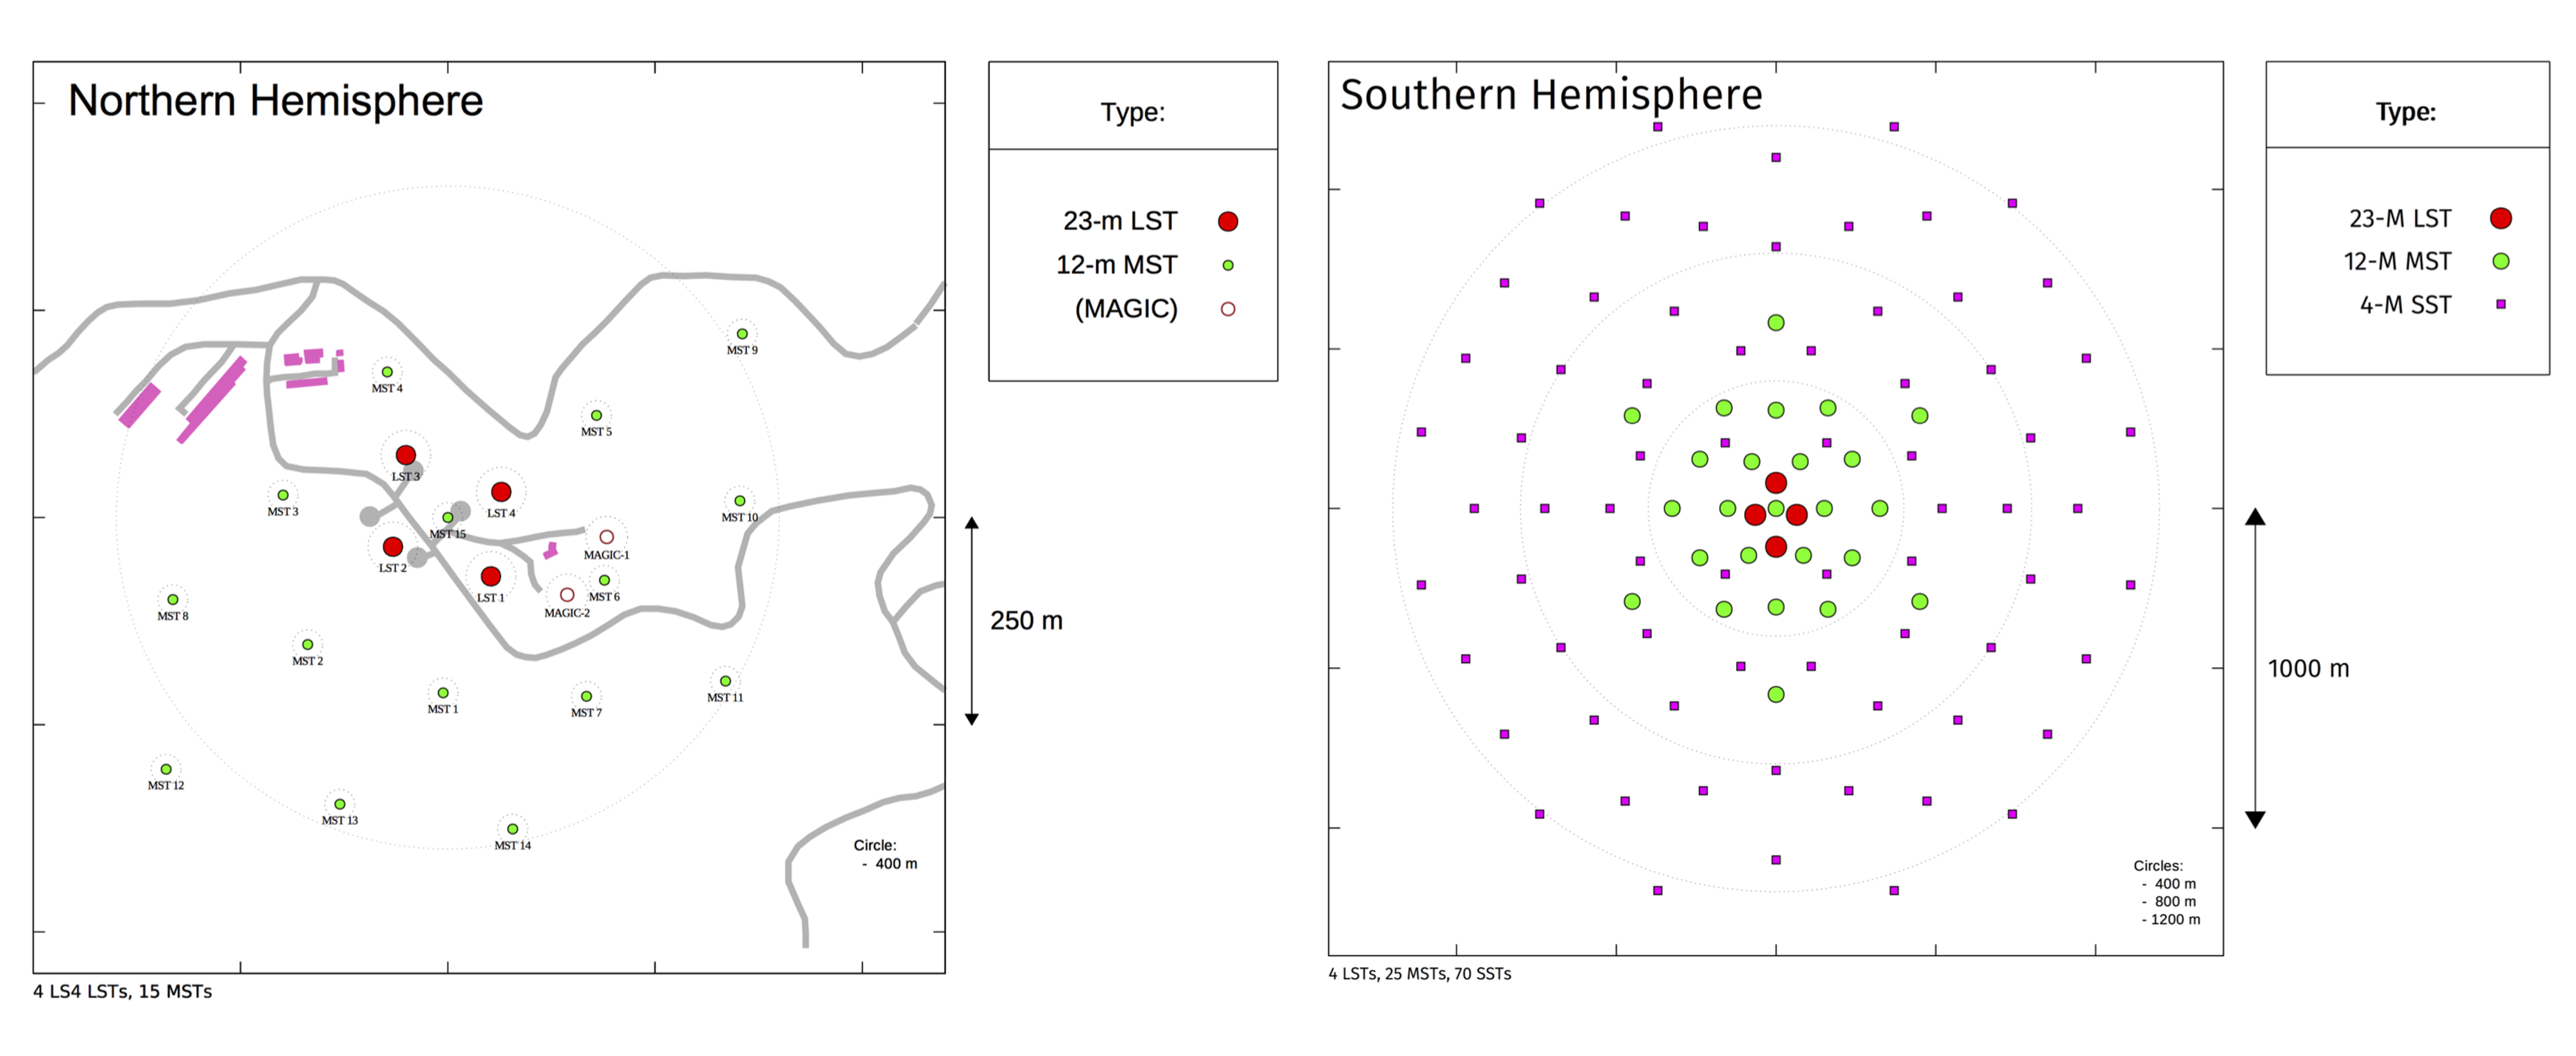
\includegraphics[width=\textwidth]{Images/ArrayLayout.png}
\caption{Der geplante Aufbau der Arrays auf La Palma und in der Atacamawüste: Auf La Palma werden zunächst nur die beiden größeren Teleskoptypen errichtet. In der Atacamawüste werden alle drei Teleskoptypten verwendet. Aufgrund der großen freien Fläche kann hier auch ein großer Bereich symmetrisch abgedeckt werden.\cite{Flickr}}
\label{img:ArrayLayout}
\end{figure}

\section{Prototyp in Adlershof}
\begin{figure}
\centering
%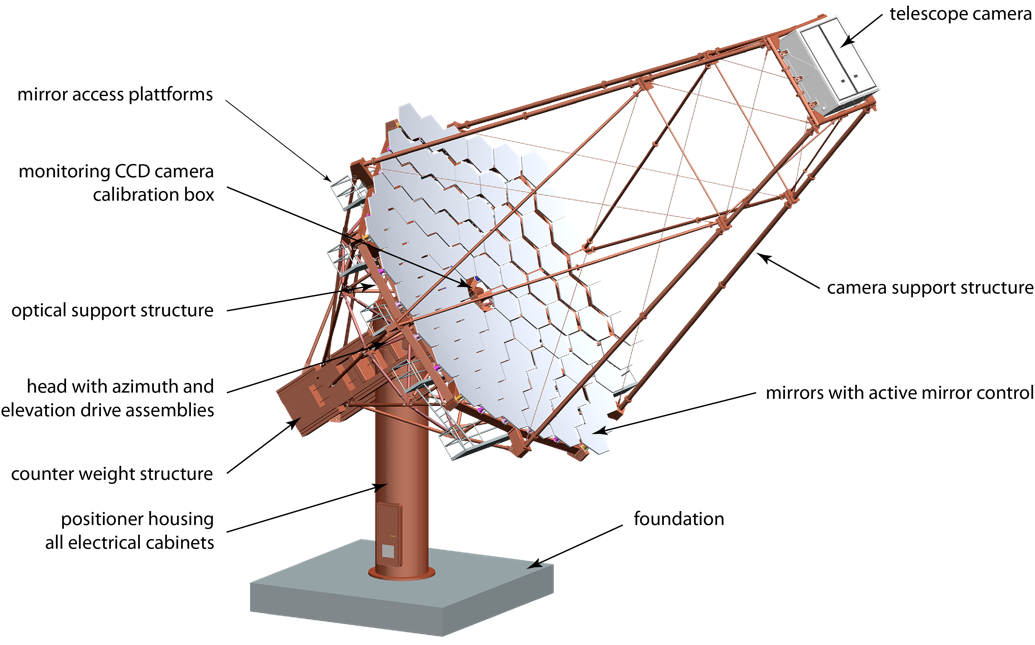
\includegraphics[width=0.5\textwidth]{Images/mst.png}
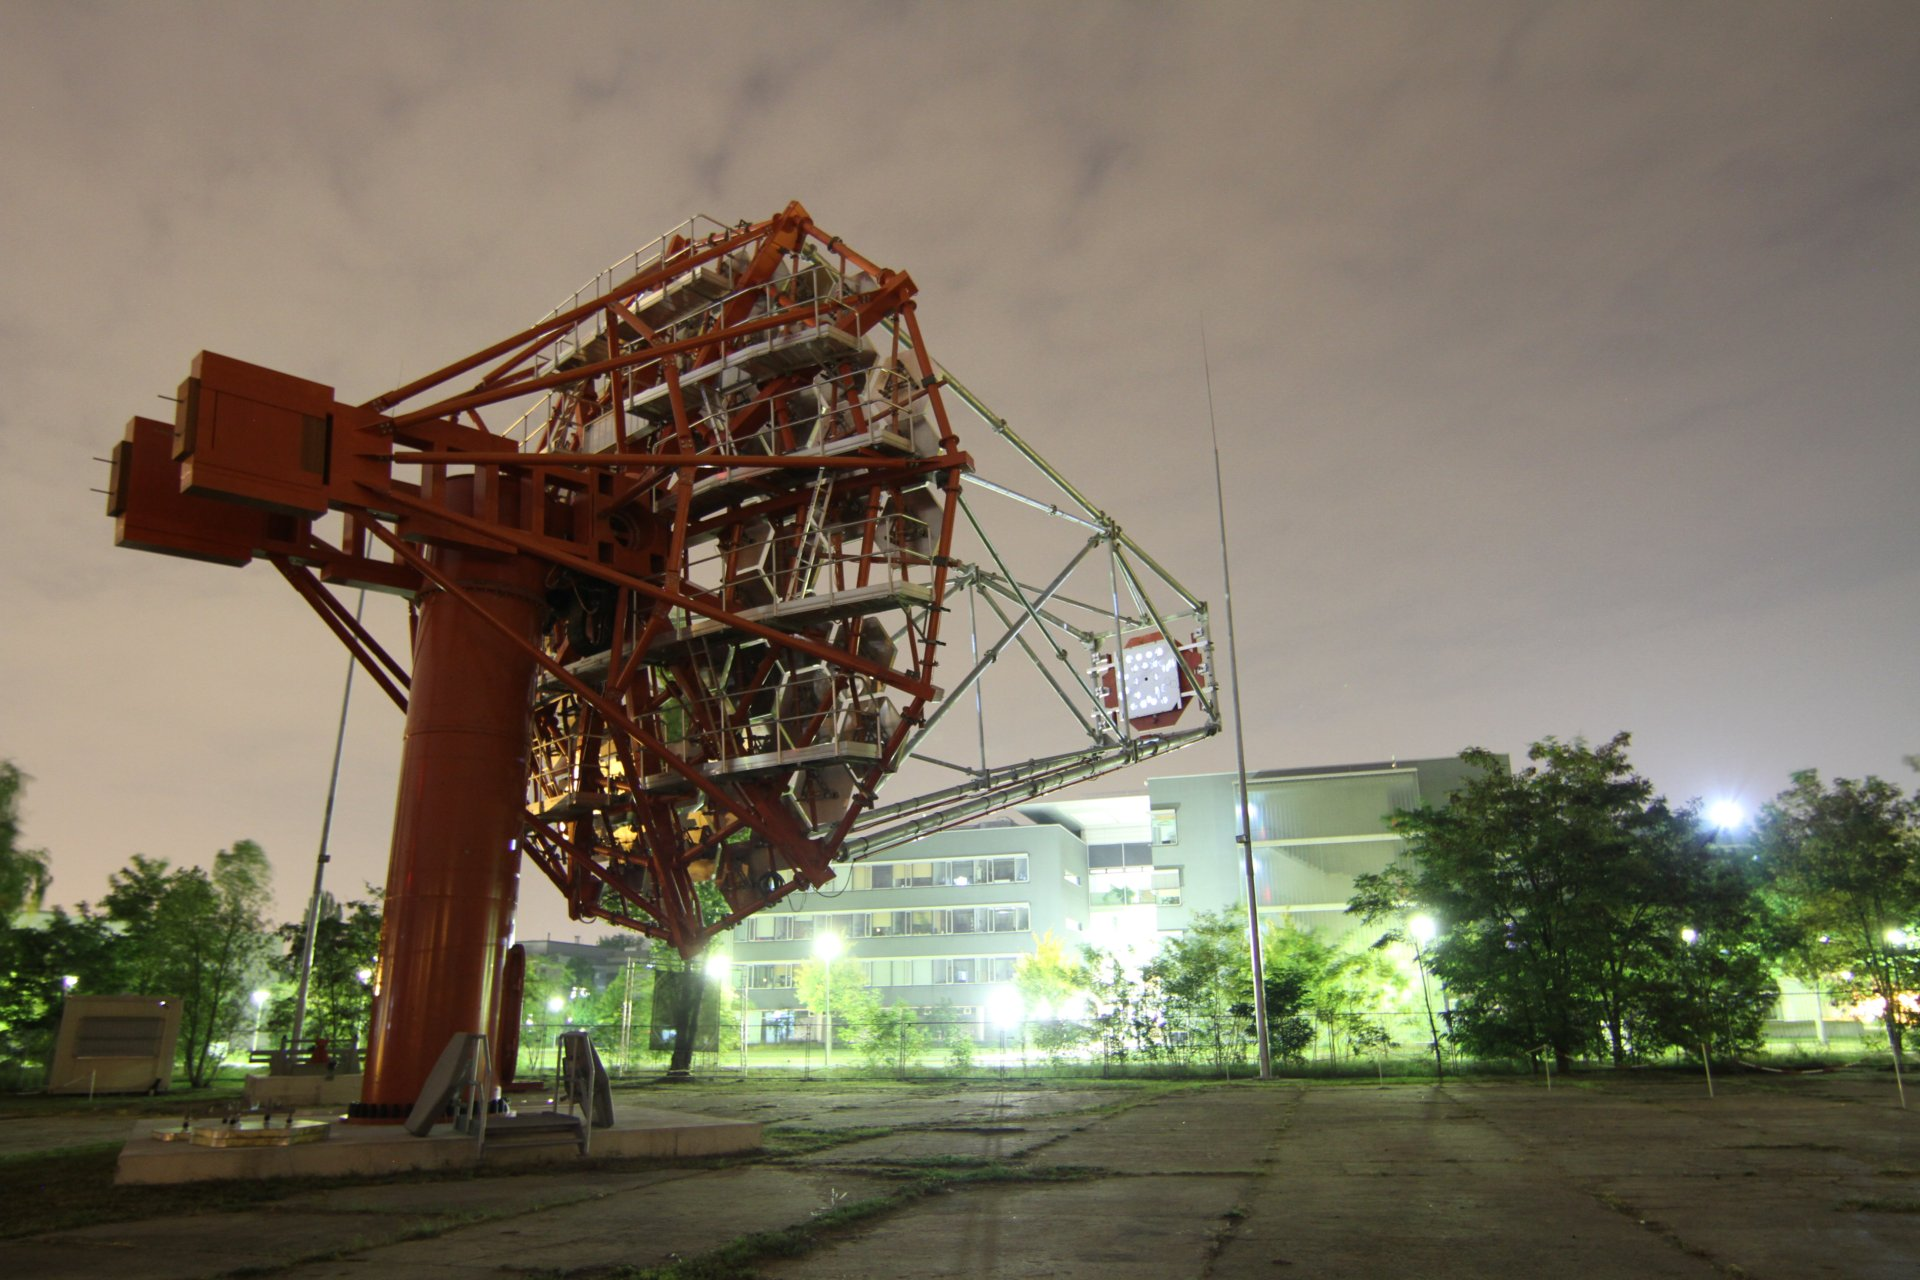
\includegraphics[width=\textwidth]{Images/night.png}
\label{img:mst}
\caption{Der Prototyp des MST in Berlin. Die Tscherenkow-Kamera wurde durch einen Dummy ersetzt und der Mitte des Reflektors befinden sich drei CCD-Kameras die in Abbildung \ref{img:cameras} besser zu sehen sind}
\end{figure}
Ein Prototyp für das MST (Abbildung \ref{img:mst}) wurde 2012 in Berlin-Adlershof in der Nähe zum DESY-Zeuthen und dem Institut für Physik der Humboldt-Universität zu Berlin errichtet. Ziel ist es mit dem Prototypen den mechanischen Aufbau zu untersuchen, die Ausrichtung der Spiegel zu testen und Pointingmethoden zu entwickeln. Dazu wurde auf eine Tscherenkovkamera verzichtet und durch einen Dummy der gleichen Masse ersetzt.

\subsection{Pointing des Teleskops mit CCD-Kameras}
Um die möglichst genaue Ausrichtung des Teleskops zu kennen verwendet man CCD-Kameras, die sowohl den Nachthimmel als auch den Dummy beziehungsweise später die Tscherenkowkamera ablichten. In sogenannten Pointing-Runs wird das Teleskop kalibriert, in dem des auf Sterne ausrichtet, deren Reflektion auf dem Dummy zu sehen ist. Mithilfe von auf dem Dummy angebrachten LEDs lässt sich die Position der Reflektion bestimmen und somit auch, wie der Dummy zum Teleskop steht. Aus den Aufnahmen vom Nachthimmel lässt sich aus der Position der zu sehenden Sterne die Koordinaten des Teleskops vorhersagen. Im Betrieb, wenn die Tscherenkowkamera geöffnet ist und die Reflektionen der Sterne nicht mehr zu sehen sind, lässt sich die Position der Tscherenkowkamera immer noch anhand der Pointing-LEDs bestimmen.

\subsection{Kameras des MST}
\label{se:cameras}
\begin{figure}
\centering
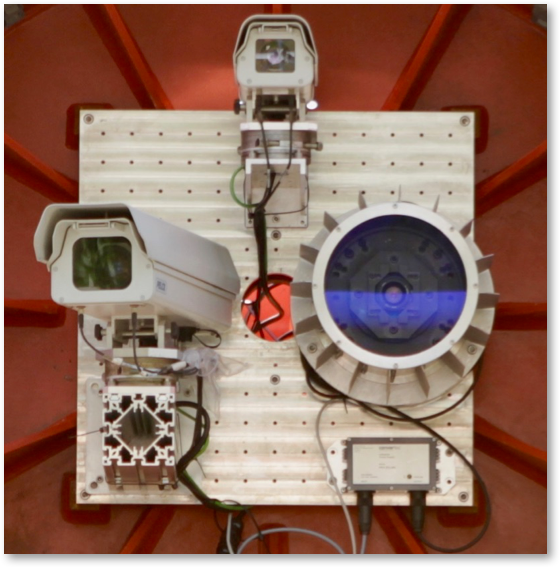
\includegraphics[width=0.5\textwidth]{Images/ccd.png}
\caption{Die drei für das Pointing verwendeten CCD-Kameras. Rechts befindet sich mit dem größten Gesichtsfeld die Single-CCD, in der Mitte oben die Lid-CCD die nur die Tscherenkow-Kamera ablichtet und links die Sky-CCD, die, wie man hier gut erkennen kann, einen großen Winkel zur optischen Achse des Teleskops hat um den Nachthimmel beobachten zu können}
\label{img:cameras}
\end{figure}
Um Pointingmodelle dieser Art zu entwickeln besitzt der Prototyp des MST drei CCD-Kameras im Zentrum des Reflektors (Abbildung \ref{img:cameras}). Die Single-CCD hat ein so großes Gesichtsfeld, dass sie gleichzeit die Tscherenkowkamera als auch den Nachthimmel ablichten kann. Alternativ können auch zwei verschiedene Kameras verwenden können, wovon eine (LID-CCD) die Tscherenkowkamera und die andere (Sky-CCD) den Nachthimmel ablichtet. Die Methode mit den beiden Kameras hat den Vorteil, dass sie zusammen eine höhere Auflösung haben. Da sich die beiden Kameras allerdings auch unabhängig voneinander bewegen können, ist die Methode mit einer CCD-Kamera das bevorzugte Konzept für das Teleskop\cite{pos}.\\
Eine Besonderheit des MST ist die Positionierung der Sky-CCD. Da sich diese wie die anderen in der Mitte des Reflektors befindet, den Dummy jedoch nicht ablichten soll, ist sie mit einem Winkel von ungefähr $10^{\circ}$ zur optischen Achse des Teleskops montiert. Wie sich die Richtung der Sky-CCD im Vergleich zu den eingestellten Koordinaten des Teleskops verhält, wird in den Kapiteln \ref{ch:pointing} und \ref{ch:auswertung} diskutiert.

\begin{table}[htbp]
\centering
\begin{tabular}{r|l}
\toprule
Modell & Prosilica GC 1350\\
Sensor & Sony ICX205\\
Auflösung & 1360 x 1024 Pixel \\
Pixelgröße & $4,65\unit{\mu m}\times 4,65\unit{\mu m}$\\
Gesichtsfeld & $4,2^{\circ} \times 3,1^{\circ} $\\
Pixel Scale & $11,03^{\circ}$\\
Bildtiefe & 8 bit\\
Objektiv & 75mm Walimex\\
\bottomrule
\end{tabular}
\caption{Technische Daten der Sky-CCD}
\label{tab:SkyCCD}
\end{table}

%In Adlershof wurde 2012 vom DESY ein Prototyp des MSTs errichtet um den mechanischen Aufbau zu testen, Pointingmodelle zu entwickeln und um die einzelnen Spiegel zu testen und auszurichten.

%\subsection{Kameras des MST}
%Der Prototyp des MST besitzt drei Kameras in der Mitte des Reflektors. Die Sky-CCD, für die im hier folgenden ein Pointingmodell entwickelt wird, ist schräg montiert, sodass sie am Detektorarm vorbei guckt um Bilder des Nachthimmels aufzunehmen. Aus diesen Bildern lassen sich mithilfe der Astrometry-Software die Koordinaten der Kamera bestimmen, die als die wahren Koordinaten angenommen werden.

%\subsection{Koordinatens des MST}
%Das MST benutzt ein Koordinatensystem aus zwei Winkeln und aehnelt den Kugelkoordinaten. Der Azimutwinkel ($az$) beschreibt die Auslenkung in der Ebenenen und lauft von $-180^{\circ}$ bis $180^{\circ}$, wobei es fuer $az=0^{\circ}$ in Richtung Norden ausgerichtet ist. Der Elevationswinkel $el$ lauft von $0^{\circ}$ bis $90^{\circ}$ wobei $el=90^{\circ}$ dem Zenit entspricht. Da es bei der Entwicklung von Pointingmodellen von Vorteil sein kann, wenn man in kartesischen Koordinaten rechnet, wurde hier die Konvention verwendet, dass Nordrichtung der x-Richtung, die Westrichtung der y-Richtung und die Zenitrichtung der z-Richtung entspricht.
%\begin{figure}[htbp]
%\centering
%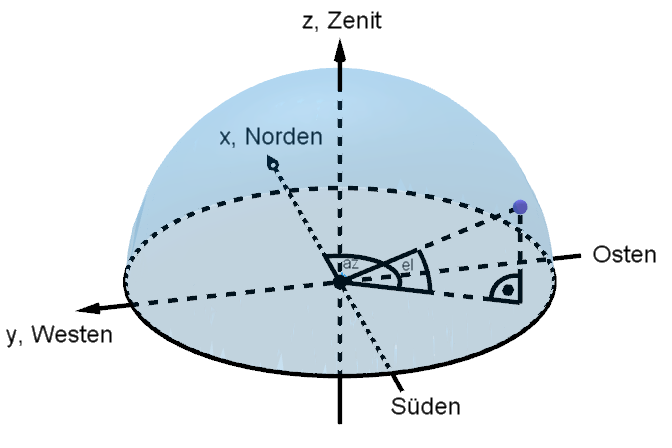
\includegraphics[width=0.7\textwidth]{Images/coordinates.png}
%\caption{Die verwendeten Koordinaten}
%\label{img:coordinates}
%\end{figure}
%\subsection{Bestimmung der Bildkoordinaten durch astronometry.net}
%Aus den mit der Kamera aufgenommen Bildern lassen sich mithilfe der astronometry.net Software die einzelnen Koordinaten der Bilder und die Groesse des Bildausschnitts bestimmen. Auf den einzelnen Bildern werden Sterne erkannt, die jeweils zu Tripplets zusammengeschlossen werden. Diese Tripletts werden mit zwei Sternenkatalogen 
%\begin{itemize}
%\item USNO-B: Ein Katalog mit ungefaehr einer Milliarde OBjekten (Sterne und Galaxien)
%\item TYYCHO-2 Ein Katalog mit den 2.5 Millionen hellsten Sternen
%\end{itemize}
%Die Software kommt auch mit Fehlern wie fehlenden und zu vielen Objekten klar.
